\newpage
\section{Hướng dẫn cài đặt, hình ảnh minh họa}

\subsection{Hướng dẫn cài đặt}
\begin{itemize}
    \item Đồ án được cài đặt trên hệ điều hành Windows 10 (hoặc Windows 11) với thư viện cURL có sẵn. Cần cài đặt thêm OpenSSL.
    \item Đường dẫn repo Github của đồ án: \href{https://github.com/ductai05/socket}{https://github.com/ductai05/socket} \cite{repo}
\end{itemize}

\paragraph{Cài đặt OpenSSL}
\paragraph{}{Để xác thực việc gửi/nhận mail, cần cài đặt OpenSSL và cài biến môi trường}
\begin{itemize}
    \item Tải Win64 OpenSSL v3.4.0 Light (\href{https://slproweb.com/products/Win32OpenSSL.html}{https://slproweb.com/products/Win32OpenSSL.html}) \\ hoặc dùng file có sẵn trong repo Github để cài đặt.
    \item Sau khi cài đặt xong OpenSSL v3.4.0, thêm \texttt{C:\textbackslash Program Files\textbackslash OpenSSL-Win64\textbackslash bin} vào PATH của biến môi trường.
\end{itemize}

\paragraph{Tải và chạy file thực thi}
\begin{itemize}
    \item Tải file nén \texttt{release.v1.0.0.zip} gồm các file \texttt{take\_screenshot.cpp, dispatcher.exe\\ server.exe} và thư mục \texttt{client} (chứa \texttt{client.exe}) từ phần \textit{releases} của repo Github: \\\href{https://github.com/ductai05/socket/releases/tag/v1.0.0}{https://github.com/ductai05/socket/releases/tag/v1.0.0} \cite{release}
    \item Thư mục \texttt{client} (chứa \texttt{client.exe}) được đặt trên máy \textbf{Client} (điều khiển). File \texttt{server.exe} và \texttt{take\_screenshot.cpp} được đặt trên các máy \textbf{Server} (bị điều khiển) và có thể có nhiều Server. File \texttt{dispatcher.exe} được đặt trên máy \textbf{Task Dispatcher} (máy điều phối). Các máy Server và máy Task Dispatcher phải được đặt trong \textbf{cùng một mạng LAN}.
    \item Thiết lập Server - Task Dispatcher, Client: các Server (\texttt{server.exe}) sẽ được chạy trước, sau đó Task Dispatcher được chạy (\texttt{dispatcher.exe}). Điều này giúp Task Dispatcher quét trong mạng LAN xem có những máy Server nào đang hoạt động. Lúc này có thể chạy Client (\texttt{client.exe}) để điều khiển các Server.
\end{itemize}

\subsection{Minh hoạ đồ án}
\subsubsection{Video thuyết trình}

\paragraph{Video Youtube thuyết trình:}
{\href{https://youtu.be/wPzeurOE8So}{https://youtu.be/wPzeurOE8So}} \cite{youtube}

\subsubsection{Hình ảnh minh họa}
%\paragraph{Hình ảnh minh hoạ}
%\paragraph{}{Sau đây là một vài hình ảnh trong game:}
\begin{figure}[H]
    \centering
    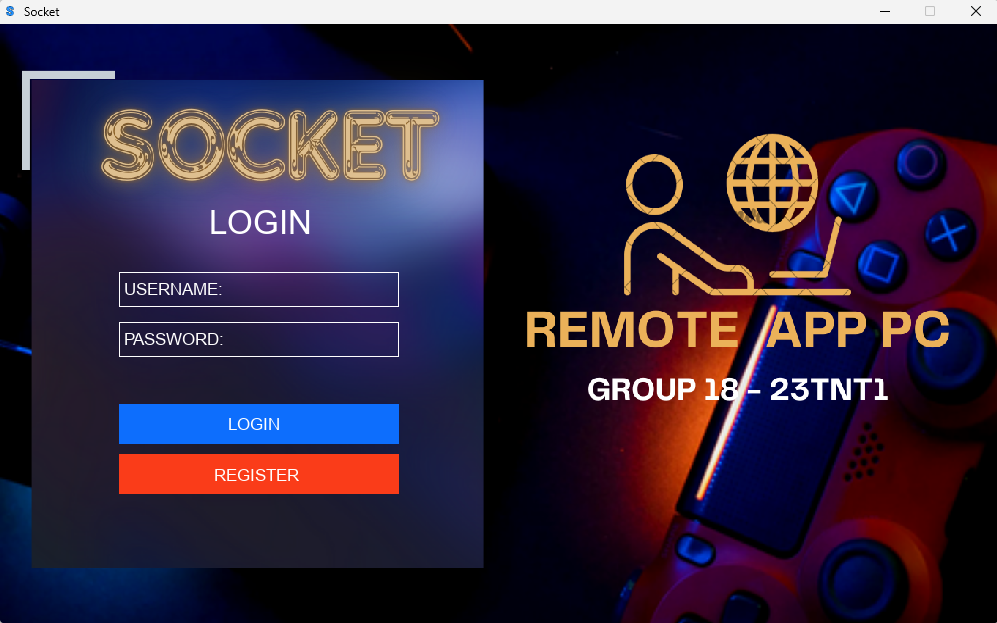
\includegraphics[width=0.89\linewidth]{img/login.png}
    \caption{Đăng nhập Client}
\end{figure}

\begin{figure}[H]
    \centering
    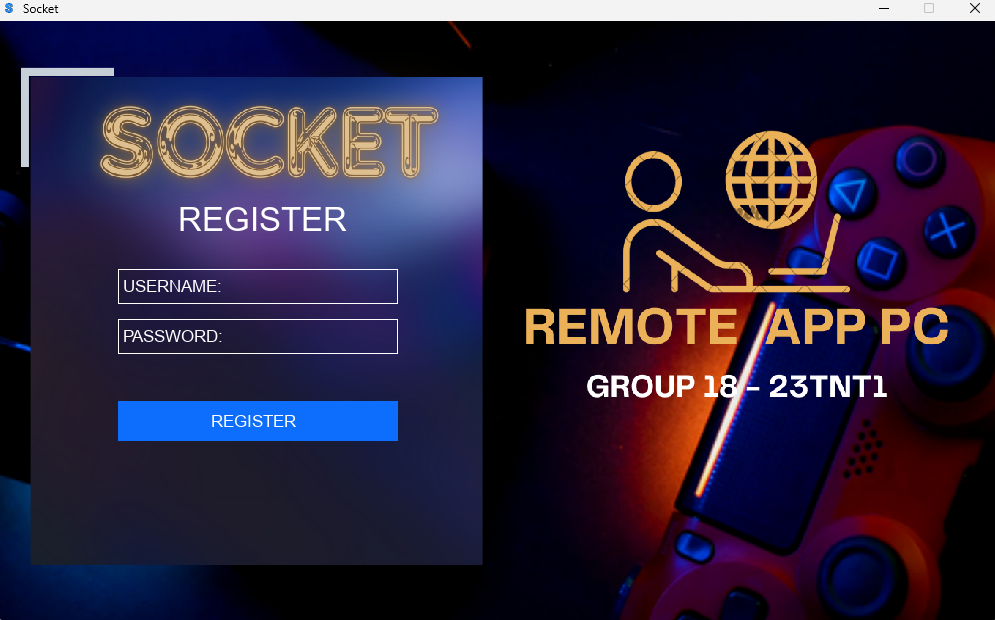
\includegraphics[width=0.89\linewidth]{img/register.png}
    \caption{Đăng kí tài khoản Client}
\end{figure}

\begin{figure}[H]
    \centering
    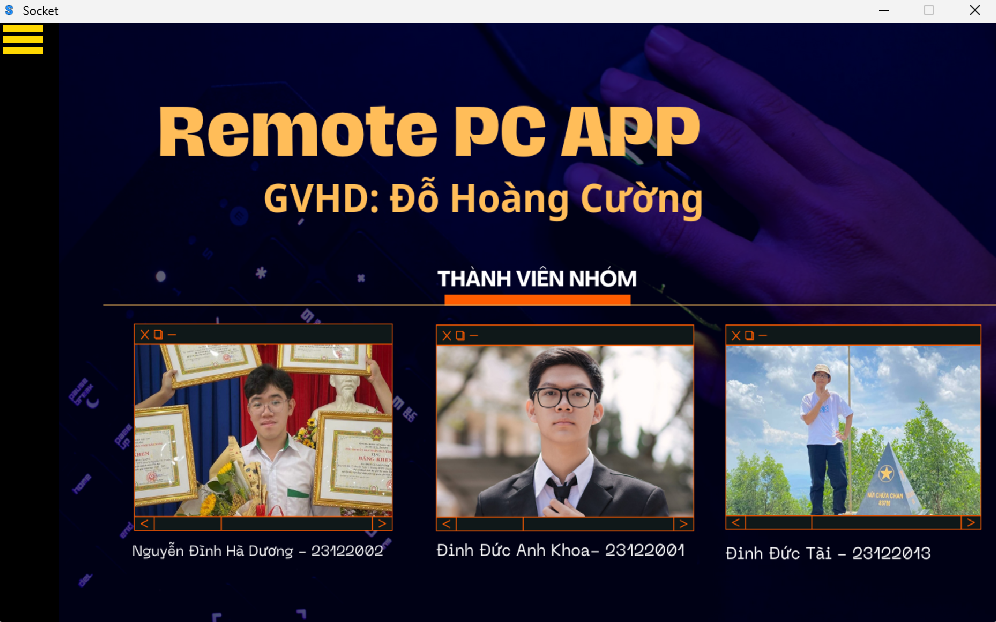
\includegraphics[width=0.93\linewidth]{img/mainpage.png}
    \caption{Giao diện giới thiệu app Client}
\end{figure}

\begin{figure}[H]
    \centering
    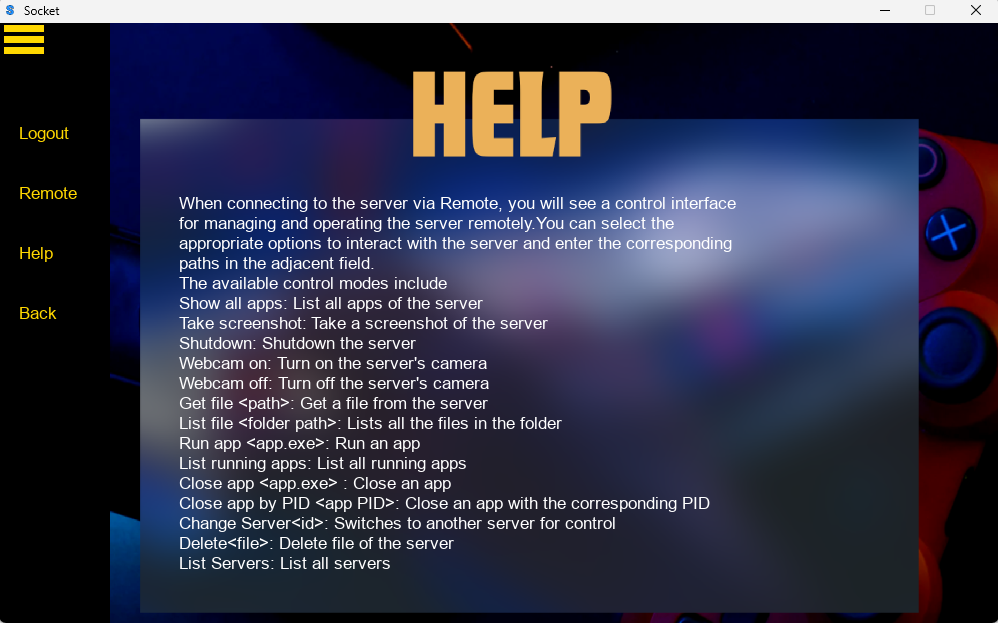
\includegraphics[width=0.93\linewidth]{img/help.png}
    \caption{Hướng dẫn sử dụng}
\end{figure}

\begin{figure}[H]
    \centering
    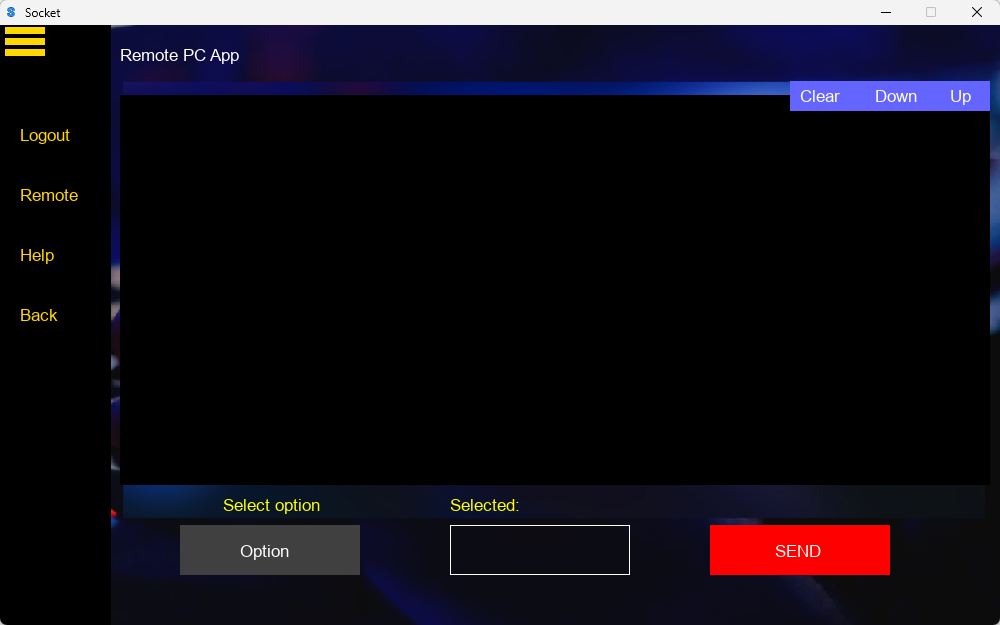
\includegraphics[width=0.93\linewidth]{img/remote.png}
    \caption{Giao diện điều khiển các Server của app Client}
\end{figure}

\begin{figure}[H]
    \centering
    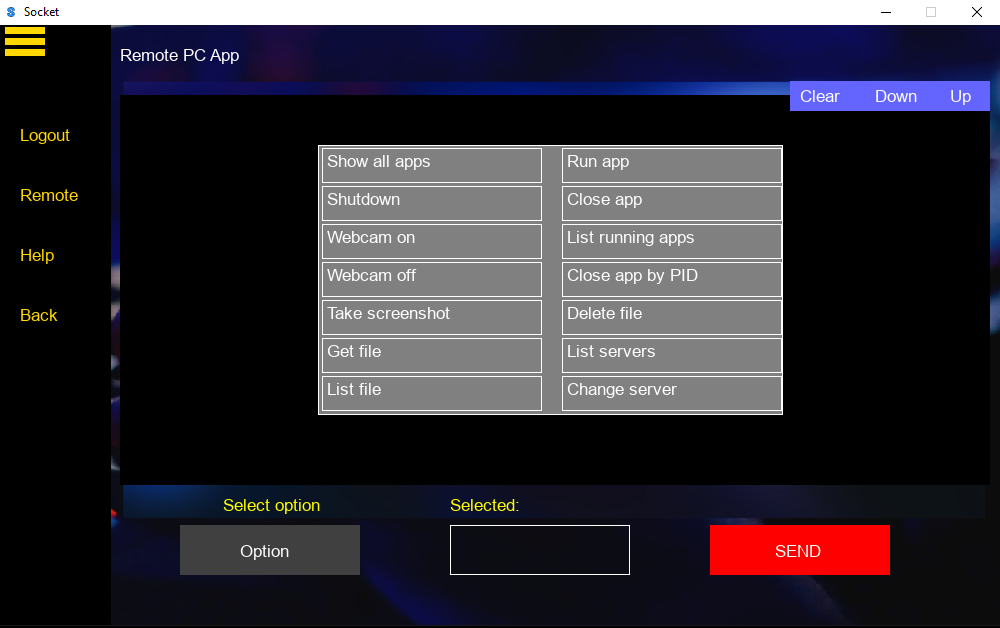
\includegraphics[width=0.93\linewidth]{img/options.png}
    \caption{Bảng lựa chọn các chức năng điều khiển}
\end{figure}

\begin{figure}[H]
    \centering
    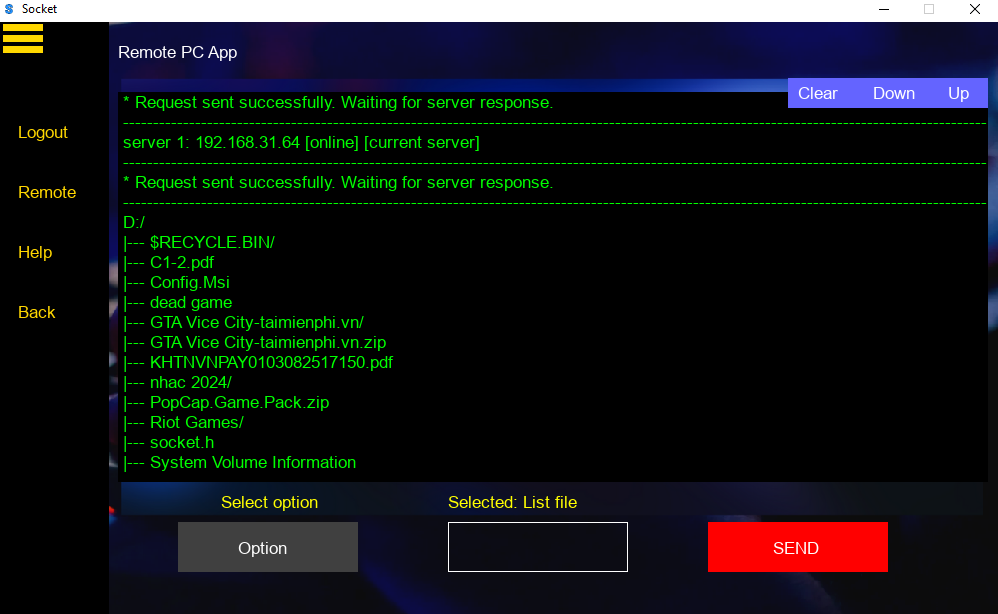
\includegraphics[width=0.93\linewidth]{img/request.png}
    \caption{Client hiển thị các thông tin được trả về từ Server}
\end{figure}

\begin{figure}[H]
    \centering
    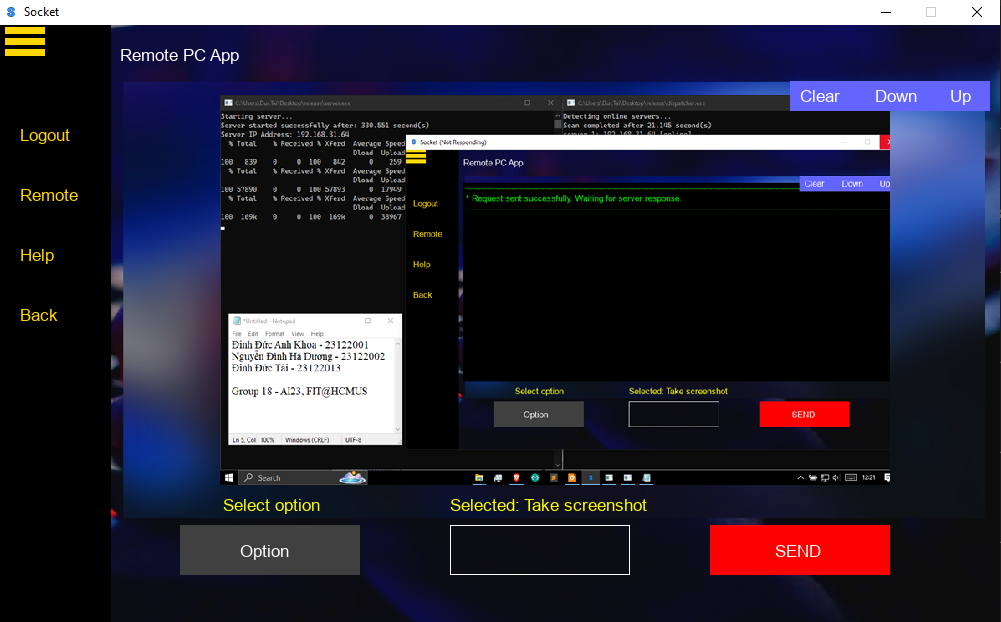
\includegraphics[width=0.93\linewidth]{img/screenshot.png}
    \caption{Client hiển thị screenshot lấy từ máy Server}
\end{figure}

\begin{figure}[H]
    \centering
    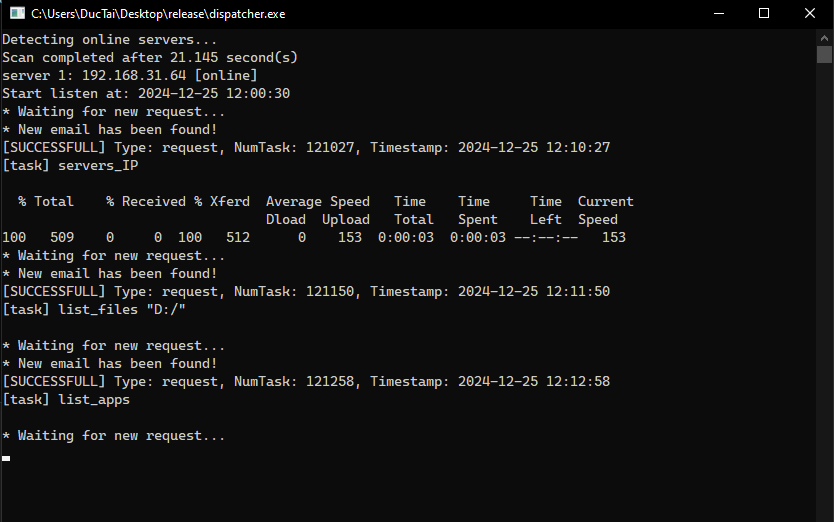
\includegraphics[width=0.93\linewidth]{img/dispatcher.png}
    \caption{Cửa sổ Console của Task Dispatcher}
\end{figure}

\begin{figure}
    \centering
    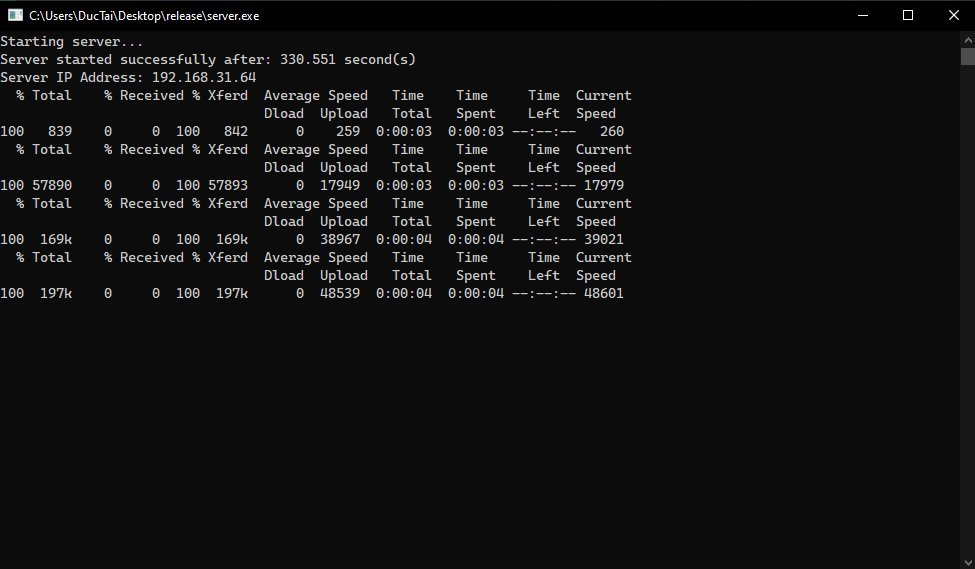
\includegraphics[width=0.93\linewidth]{img/server.png}
    \caption{Cửa sổ Console của Server}
\end{figure}